\documentclass[12pt,a4paper]{article}
\usepackage[T2A]{fontenc}
\usepackage[utf8]{inputenc}
\usepackage[english,russian]{babel}
\usepackage{amsmath}
\usepackage{graphicx}
\usepackage{booktabs}
\usepackage[margin=22mm]{geometry}
\usepackage[unicode,hidelinks]{hyperref}

\title{Пример LaTeX}
\author{}
\date{}

\begin{document}
\maketitle

\section{Формула}
Пусть $n_i$ обозначает число объектов категории $i$, а всего категорий $k$
Доля категории определяется как
\begin{equation}
    p_i = \frac{n_i}{\sum_{j=1}^{k} n_j},
    \qquad \sum_{j=1}^{k} n_j > 0
    \label{eq:share}
\end{equation}
В формуле~\eqref{eq:share} знаменатель содержит общее число объектов

При пустом наборе доля по этой формуле не определена

\section{Рисунок}
Примеры преобразования документов показаны на рисунке~\ref{fig:workflow}
\begin{figure}[ht]
    \centering
    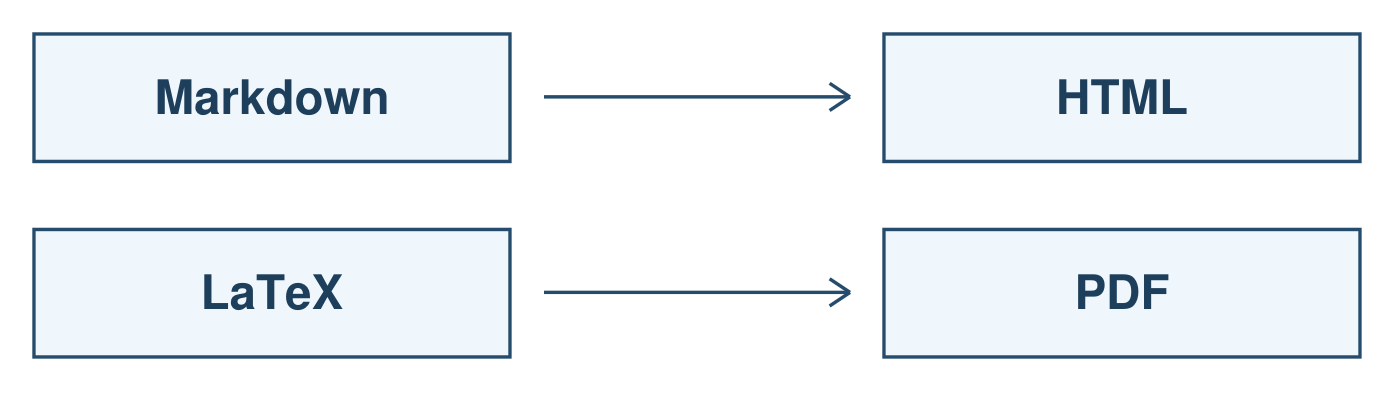
\includegraphics[width=\linewidth]{workflow.png}
    \caption{Примеры преобразования документов}
    \label{fig:workflow}
\end{figure}

\section{Таблица}
\begin{center}
\begin{tabular}{ll}
\toprule
Формат & Результат \\
\midrule
Markdown & HTML \\
LaTeX & PDF \\
\bottomrule
\end{tabular}
\end{center}

\end{document}
